\documentclass{article}
\usepackage{setspace}
\usepackage{geometry}
\usepackage[utf8]{inputenc}
\usepackage{amsmath,amsthm,amssymb,bm}
\usepackage{mathtools}

\geometry{letterpaper, portrait, margin=1in}
\setstretch{1.5}
\title{Homework 9}
%\date{1-18-2020}
\author{Runmin Lu}

\begin{document}
	\maketitle
	%\newpage
	
	\section*{1}
		$Z$ has dimension $N \times 45 = N \times \sum\limits_{i=0}^8(i+1)$ because for each power $i$ from 0 to 8 we have $i+1$ combinations of $x$ and $y$ and $N$ is the number of data points.
	
	\section*{2}
		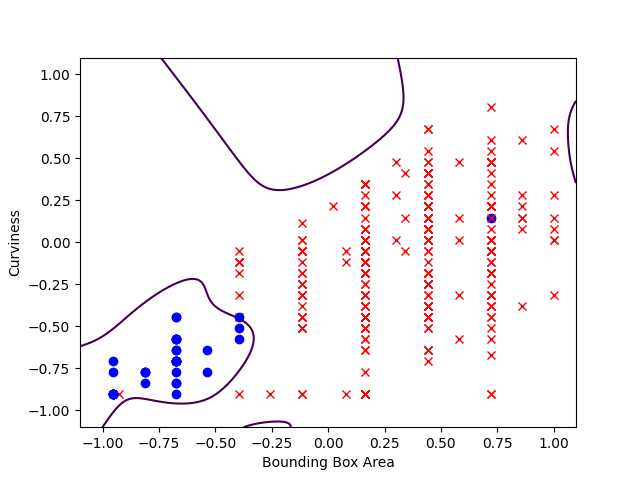
\includegraphics[scale=0.8]{2.png}\\
		There is overfitting because the top boundary doesn't make sense. Something more curvy should not be more likely to be a 1.
	\section*{3}
		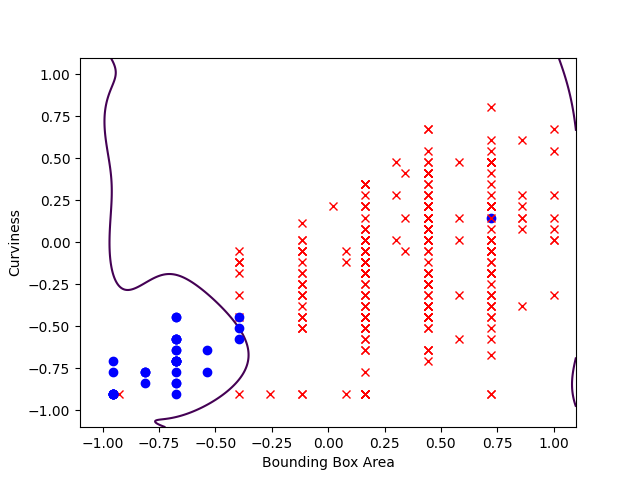
\includegraphics[scale=0.8]{3.png}\\
		There is still overfitting but less. The upper right boundary doesn't make sense for the same reason.
	\section*{4}
		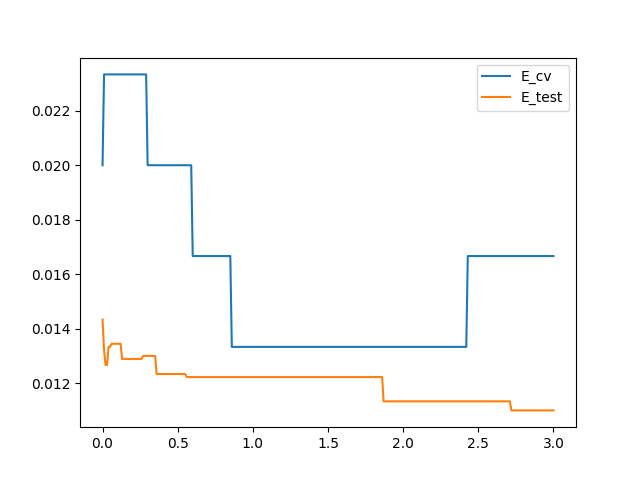
\includegraphics[scale=0.8]{4.png}\\
		$E_\text{cv}$ is close to $E_\text{test}$. The gap looks large because it's zoomed in and the $y$-axis doesn't start at 0 but if you look at the numbers, it's actually pretty small.
		
	\section*{5}
		$\lambda^* = 2.42$\\
		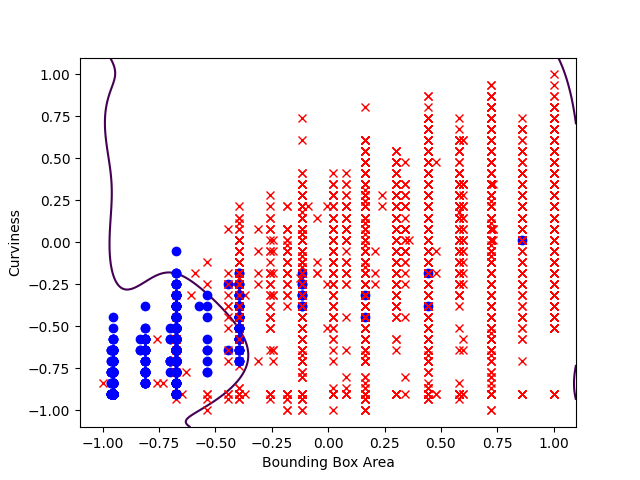
\includegraphics[scale=0.8]{5.png}
		
	\section*{6}
		\begin{align*}
			E_\text{test}(\mathbf w_\text{reg}(\lambda^*)) &\approx 0.0111\\
			E_\text{out}(\mathbf w_\text{reg}(\lambda^*)) &\leq E_\text{test}(\mathbf w_\text{reg}(\lambda^*)) + \sqrt{\frac1{2 \times 8998}\ln \frac2{0.01}}\\
			&\approx 0.0111 + 0.0172\\
			&= 0.0283
		\end{align*}
		
	\section*{7}
		No because we use $E_\text{cv}(\lambda^*)$ to select $\lambda^*$, which is then used to select $\mathbf w_\text{reg}(\lambda^*)$ as the final hypothesis. That's where data snooping occurs. On the other hand, $E_\text{test}(\mathbf w_\text{reg}(\lambda^*))$ purely measures the performance of $\mathbf w_\text{reg}(\lambda^*)$ because we do not use the test set $\mathcal D_\text{test}$ in training at all.
		
	\section*{8}
		Yes because there's no data snooping. $E_\text{test}(\mathbf w_\text{reg}(\lambda^*))$ uses $\mathcal D_\text{test}$ to evaluate the performance of $\mathbf w_\text{reg}(\lambda^*)$, which in no way affected the selection of $\mathbf w_\text{reg}(\lambda^*)$. The selection only use the 300 data points in a completely separate set $\mathcal D$.
		
\end{document}